\section{Probabilistic Trace Alignment as a $k$NN Problem}\label{sec:topk}
Trace alignments algorithms provide as output a single alignment from a single model trace. This is not very convenient in practice because rich feedback should provide different possibilities. This is even more important when the Workflow Nets (such as USWNs) are stochastic, and the different model traces have different probabilities. {Instead, we would like to return the best $k$ alignments among all the possible unravelled traces from the USWN $\mathcal{U}$. If we want to produce the best $k$ alignments from $\mathcal{U}$ for a trace $\sigma^*$, the approach described in the previous section requires to visit the entire search space $\mathcal{W}_{p_\theta}^n(P)$ where $P$ is the TG associated to $\mathcal{U}$. On the other hand, we prefer to reduce the search space by starting the visit from the traces nearer to $\sigma^*$.}


%\texttt{\color{red}[TODO: introduction, motivation, and why it is useful to run it as a $k$-best search]}
%\resizeableyellownote{3}{3}{
%	Assuming that Rafael writes the definition of his ranking function, that can be expressed as $r(\sigma^*,\sigma)=d(\sigma^*,\sigma)w_\sigma$ for a query trace $\sigma^*$ and a trace $\sigma\in\mathcal{W}_p^n(P)$
%}

$k$-nearest neighbors ($k$NN) is a well-known problem in database theory \cite{Altman} which has the goal of finding the $k$ nearest data points to a query $x$ from a set $\mathcal{X}$ of data points via a distance function $d$ defined over $\mathcal{X}\cup\{x\}$. {If the query  $x$ is performed over ad-hoc data structures (Vp-Trees \cite{Fu2000}, Kd-Trees \cite{Maneewongvatana99}, and M-Trees \cite{Ciaccia}), then we can straight identify the nearest neighbors of $x$ in $\mathcal{X}$ (without analyzing the entire space) by pre-ordering $\mathcal{X}$ within the data structure of choice via $d$. This characterization could be exploited for top-$k$ trace alignments: if $x$ is the trace $\sigma^*$ that we want to align over the unraveled traces $\mathcal{X}=\mathcal{W}^n_{p_\theta}(P)$ and $d$ is a distance defined for probabilistic traces, then $k$-nearest neighbors describe the best $k$ alignments for $\sigma^*$.}
	
{For the aforementioned data structures, $x$ (and $\mathcal{X}$) is usually represented as a (set of) vector(s) via embedding  $\phi$, while the distance $d$ can be either the Euclidean distance or an ad-hoc vector distance $d_{k_\phi}$ defined over $k_\phi$ (see Equation \ref{eq:dofk}). $\phi$ is chosen to be independent from the query $x$, so that all the vectors $\phi(x_i)$ for $x_i\in\mathcal{X}$ are not changed for each new query $x$.}

%\begin{figure}[!t]
%	\centering
%	\subfloat[The similarity/probability space.]{\label{fig:spp}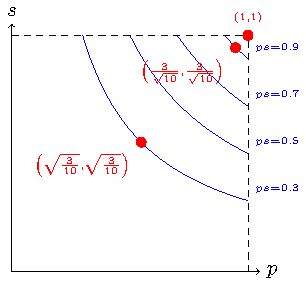
\includegraphics[width=.45\textwidth]{images/original_space.pdf}}\qquad
%	\subfloat[The transformed space for the $k$ nearest neighbours problem.]{\label{fig:knnspace}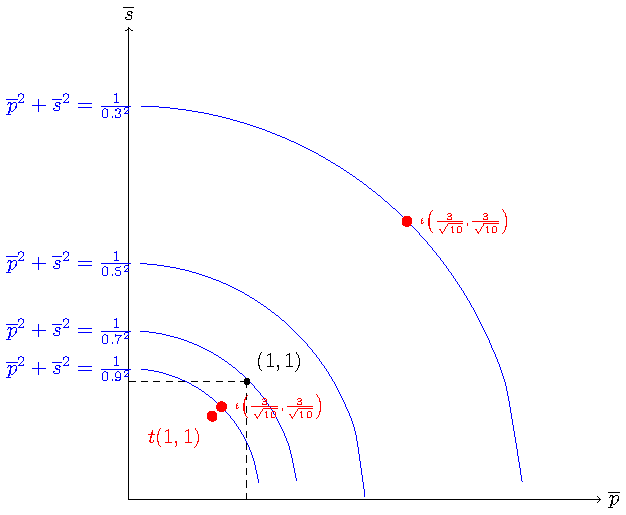
\includegraphics[scale=0.55]{images/transformed_space.pdf}}\\
%	\caption{Two different characterizations of the probabilistic trace alignment problem. The best possible match is represented in red in both the %similarity/probability space and in the transformed one.}
%\end{figure}
\ADD{The Approximate-Ranking Trace Embedder } meets the $k$NN desiderata as $\phi_{\mathcal{P}}$ is defined independently from $\sigma^*$: \ADD{by exploiting the aforementioned data structures, we can retrieve the top-$1$ alignment according to $k_{\phi_\mathcal{P}}$ by traversing the preloaded data structure at most with an initial logarithmic look-up search and, starting from this alignment, we can visit the neighborhood for retrieving the remaining $k-1$ traces. 

On the other hand, the} $k_\star$ \ADD{associated to the Optimal-Ranking trace aligner} is tightly bounded to the specific $\sigma^*$ of choice via the alignment cost $d$, \ADD{thus implying that retrieving the top-$1$ trace still requires a preliminary linear visit of all the traces in $\mathcal{X}$} In order to maximise the decoupling of the vectorial representation from $\sigma^*$ with $w_{\sigma^*}=1$,
 we can embed each unravelled trace $\braket{\sigma,w_\sigma}$ via $\phi_\star(\braket{\sigma,w_\sigma})=\Big(\frac{1}{w_\sigma\sqrt{w_\sigma^2+s_d^2(\sigma,\sigma^*)}},\frac{1}{s_d(\sigma,\sigma^*)\sqrt{w_\sigma^2+s_d^2(\sigma,\sigma^*)}}\Big)$ (Figure \ref{fig:knnspace}) and the query trace $\sigma^*$ to $x=(0,0)$, so that the the Euclidean distance between the vector of an unravelled trace in $\mathcal{X}$ and the origin $x$ is  inversely proportional to $k_\star(\sigma,\sigma^*)$. The proof is omitted due to lack of space. \ADD{Contrary to what happens for $\phi_{\mathcal{P}}$, $\phi_\star$ requires to pay a linear scanning cost for generating the new set of vectors for each new query trace  $\sigma^*$ before performing the top-$1$ look-up in the transformed space (Figure \ref{fig:knnspace}).}

\begin{example}
	Figure \ref{fig:spp} shows a family of hyperbolae $w_\sigma s(\sigma,\sigma^*)=k$ describing all the points $(w_\sigma, s(\sigma,\sigma^*))$ having $k$ as a $k_\star$ score. Point $\color{red}(1,1)$ represents the best possible trace match, as it means that there exists a trace $\braket{\sigma^*,1}\in\mathcal{W}_{p_\theta}^n(P)$.
		Figure \ref{fig:knnspace} shows that the aforementioned embedding moves the points of the hyperbola $w_\sigma s(\sigma,\sigma^*)=k$ over a circumference $x^2+y^2=\sfrac{1}{k^2}$ describing a locus of the points equidistant from the origin of the axes $(0,0)$ with distance $\sfrac{1}{k}$: this intuitively means that the $k$NN algorithm will first visit the points nearer to the origin by picking up the nearest circumference, and then will visit the next circumference.
\end{example}

%\xout{In particular, we want to exploit the well-known \textit{k}-nearest neighbour problem for providing this desired result. Such problem can be formalized as follows:}
%\begin{definition}[$k$-Nearest Neighbour]
%	\xout{Given a set of vectors  $\mathcal{X}\subseteq \mathbb{R}^d$ within a $d$-dimensional Euclidean space and a query vector $q\in\mathbb{R}^d$, the $k$-nearest neighbour algorithm returns a subset $K\subseteq\mathcal{X}$ of $k$ elements minimizing the distance from $v$:}
%	$$\Rcancel{knn_\delta(k,q,\mathcal{X})=\begin{cases}
%	\emptyset& k \leq 0\\
%	\{c\}\cup knn(k-1,q,\mathcal{X}\backslash\{c\}) & k> 0 \Rightarrow c:={\arg\min}_{x\in\mathcal{X}}\delta(x,q)\\
%	\end{cases}}$$
%	\xout{where $\delta$ is a distance measure between the vectors.}
%\end{definition}
%{While for the proposed approximate trace embedder we can directly use this formulation by exploiting an embedding $\phi_{\mathcal{P}}$ and a distance $d(\sigma,{\sigma^*})=1-k_{\phi_\mathcal{P}}(P_\sigma,P_{\sigma^*})$ \xout{for $k_{\phi_\mathcal{P}}(P,P')$ returns $1$ as a maximum value}, the price that we need to pay if we want to exploit the existing aligners is alignment cost for all the unravelled traces in $\mathcal{X}$. In fact, we can either directly exploit $k_\star$ and the fact that kernels can be always expressed as distance functions $d_{k_\star}$ \cite{Gartner03}, or we need to transform each unravelled trace $\braket{\sigma,w_\sigma}$ as a point $(x,y)\in\mathbb{R}_{\geq 0}^2$ and the to-be-aligned trace $\sigma^*$ as an arbitrary vector $(0,0)$, so that the Euclidean distance between the two associated vectors is proportional to $d_{k_\star}$. Given that the ordering of the traces depends on trace to be aligned, this implies to either re-sort the data all the time or to re-compute the associated embedding from scratch.}
%
%\subsection{Exact $k$-probabilistic Traces Alignment Problem}\label{subsec:exbkptap}
%%\texttt{\color{red}[TODO: the introduction of this section depends on how we want to formulate the problem. I suddenly start with the definition of the k-Nearest Neighbour, but I am aware that we need to provide first a bit of context]}
%
%
%
%\xout{In order to reduce the exact probabilistic trace alignment problem to the \textit{k}-nearest neighbour, we can first map each weighted trace  $\braket{\sigma,w_\sigma}\in\mathcal{W}_p^n(P)$ that we need to align with $\sigma^*$ as a point $\sigma\overset{\mu_{\sigma^*}}{\mapsto}(w_\sigma,\; s_d(\sigma,\sigma^*))$ in the 2-dimensional similarity/probability space of coordinates $(p,s)$, so that the trace finding problem reduces to find a data point maximising the product $p\cdot s\equiv w_\sigma\cdot s_d(\sigma,\sigma^*)$ (Figure \ref{fig:spp}).}
%
%%\begin{table}[!t]
%%\centering
%%\caption{Expected ranking of the paths from Example \ref{ex:withpaths} with the trace $\sigma^*=\textup{caba}$. The cost function is the one from \cite{LeoniM17} and its normalized similarity score has $c=5$.}\label{tab:expected}
%%\begin{tabular}{lc|ll|cl}
%%	\toprule
%%	
%%	\multirow{2}{*}{$\sigma$} &
%%	\multirow{2}{*}{$d(\sigma,\sigma^*)$} &
%%	\multicolumn{2}{c|}{$\mu_{\sigma^*}$} &
%%	 \multirow{2}{*}{$\approx s_d(\sigma,\sigma^*)\cdot w_\sigma$} & \multirow{2}{*}{\textit{expected ranking}}\\
%%	
%%	\cline{3-4} &&  $\langle w_\sigma$ &  $,\,s_d(\sigma,\sigma^*)\rangle $ &&\\
%%	
%%	\midrule
%%	{a}  & $3$ & $0.4$ & $\;\; 0.6250$  & $0.2500$ & \textbf{1}\\
%%	{aa}  & $2$ & $0.2$ & $\;\; 0.7142$ & $0.1428$ & \textbf{2}\\
%%	{aaa}  & $2$ & $0.1$ & $\;\; 0.7142$ & $0.0714$ & \textbf{3}\\
%%	{ca}  & $2$ & $0.07$ & $\;\; 0.7142$ & $0.0500$ & \textbf{4}\\
%%	{cb}  & $2$ & $0.06$ & $\;\; 0.7142$ & $0.0428$ & \textbf{5}\\
%%	{aaaa}  & $3$ & $0.05$ & $\;\; 0.7142$ & $0.0357$ & \textbf{6}\\
%%	{caa}  & $1$ & $0.035$ & $\;\; 0.8333$ & $0.0292$ &  \textbf{7}\\
%%	{caaa}  & $1$  & $0.0175$ & $\;\; 0.8333$ & $0.0145$ & \textbf{8}\\
%%	\bottomrule
%%\end{tabular}
%%\end{table}
%\begin{example}\label{ex:rankingTaus}
%\xout{Table \ref{tab:expected} represents the expected exact alignment raking of all the weighted traces $\braket{\sigma,w_\sigma}\in\mathcal{W}_0^4(P)$ generated by the TG $P$ in Figure \ref{3figs} with a trace $\sigma^*=\textup{caba}$.  Albeit traces \textit{caa} and \textit{caaa} are the most similar with \textit{caba}, their associated trace probability is $w_\sigma$ is rather low, so traces having higher probability but lower similarity score are preferred (e.g., \textit{a} and \textit{aa}). Given that users might still prefer the most similar ones to the ones maximising both probability and similarity, we prefer to offer the user the whole set of the best $k$ solutions rather than cherry-picking the best solution maximising both probability and similarity.}
%\end{example}
%
%\xout{After this preliminary step, we can finall reduce the problem into the desired $k$-nearest neighbour by exploiting $\delta$ as the usual Euclidean Distance. In order to do so, we define a transformation $t$ such that the distance of $t(p,s)$ towards  the origin of the axes $\vec{0}$ (representing the trace to be aligned $\sigma^*$) corresponds to $\sfrac{1}{ps}$, so the transformed data points maximising $ps=k$ are all at the same distance $\sfrac{1}{k}$ from $\vec{0}$ (Figure \ref{fig:knnspace}). A possible transformation is the following:}
%\[t(p,s):=\left(\frac{1}{s\sqrt{p^2+s^2}},\; \frac{1}{p\sqrt{p^2+s^2}}\right)\]
%
%
%
%
%
%
% \xout{We can show with the next lemma that the following transformation is the one reducing the problem to the $k$-Nearest Neighbour problem:}
%
%
%
%\begin{lemma}
%\xout{Given a value $k\in[0,1]\subseteq \mathbb{R}^+_0$, the set of points having the product $ps$ at least $k$ corresponts to the set of $t$-transformed points having a distance of at least $1/k$ from the origin of the axes.}
%\end{lemma}
%\begin{proof}
%\[\begin{aligned}
%ps\geq k&\Rcancel{\Leftrightarrow \frac{1}{ps}\leq\frac{1}{k}} \\
%	   &\Rcancel{\Leftrightarrow \frac{\sqrt{p^2+s^2}}{ps\sqrt{p^2+s^2}}\leq\frac{1}{k} }\\
%	   &\Rcancel{\Leftrightarrow \sqrt{\frac{p^2+s^2}{p^2s^2(p^2+s^2)}}\leq\frac{1}{k}} \\
%	   &\Rcancel{\Leftrightarrow \sqrt{\frac{p^2}{p^2s^2(p^2+s^2)}+\frac{s^2}{p^2s^2(p^2+s^2)}}\leq\frac{1}{k}} \\
%	   &\Rcancel{\Leftrightarrow \sqrt{\frac{1}{s^2(p^2+s^2)}+\frac{1}{p^2(p^2+s^2)}}\leq\frac{1}{k}} \\
%	   &\Rcancel{\Leftrightarrow \left\|{\biggr({\frac{1}{s\sqrt{p^2+s^2}},\frac{1}{p\sqrt{p^2+s^2}}\biggr)}-\vec{0}}\right\|_2\leq\frac{1}{k}} \\
%	   &\Rcancel{\Leftrightarrow \left\|t(p,s)-\vec{0}\right\|_2\leq\frac{1}{k}} \\
%\end{aligned}\]
%\end{proof}
%\begin{lemma}
%\xout{Given a Workflow Net $P$ and a trace $t^*$, the probabilistic trace alignment problem of the best $k$ traces reduces to the $k$-Nearest Neighbour problem $\mu_{\sigma^*}^{-1}(knn(k,\vec{0},\mu_{\sigma^*}(\mathcal{W}_0^{\aleph_0}(P))))$.}
%\end{lemma}
%\begin{proof}
%\xout{Trivial by definition of $\mu_{\sigma^*}$ and for the previous lemma.}
%\end{proof}
%
%%\begin{table}[!t]
%%\centering
%%\caption{Representing the point from Table \ref{tab:expected} in the transformed space.}\label{tab:transf}
%%\begin{tabular}{ll|lll}
%%	\toprule
%%	
%%	$\sigma$ & $t(\mu_{\sigma^*}(\sigma))$ & $\norm{t(\mu_{\sigma^*}(\sigma))-\vec{0}}{2}$ & $\frac{1}{\norm{t(\mu_{\sigma^*}(\sigma))-\vec{0}}{2}}$ & \textit{distance ranking}\\
%%	
%%	\midrule	
%%	a   & $\braket{2.16, \;\,3.37}$ & $4.00$ & $0.2500$ & \textbf{1}\\
%%	{aa}  & $\braket{1.89, \;\,6.74}$ & $7.00$ & $0.1428$ & \textbf{2}\\
%%	aaa   & $\braket{1.94, 13.87}$ & $14.00$ & $0.0714$ & \textbf{3}\\
%%	ca   & $\braket{1.95, 19.91}$ & $20$ & $0.0500$ & \textbf{4}\\
%%	{cb}  & $\braket{1.95, 23.25}$ & $23.33$ & $0.0428$ & \textbf{5}\\
%%aaaa   & $\braket{1.95, 27.93}$ & $28.00$ & $0.0357$ & \textbf{6}\\
%%caa   & $\braket{1.44, 34.26}$ & $34.29$ & $0.0292$ & \textbf{7}\\
%%caaa   & $\braket{1.44, 68.56}$ & $68.57$ & $0.0145$ & \textbf{8}\\
%%	\bottomrule
%%\end{tabular}
%%\end{table}
%\begin{example}
%\xout{We now want to show the correctness of the former lemmas with some examples.
%Table \ref{tab:transf} represents the transformed points $t(\mu_{\sigma^*}(\sigma))$ from the data points $\mu_{\sigma^*}(\sigma)$  calculated  Example \ref{ex:rankingTaus}. The third column shows the distance of the transformed point from the origin: the following column shows that the inverse of such distance exactly represents the previously calculated $s_d(\sigma,\sigma^*)\cdot w_\sigma$, thus empirically implying that the $k$-nearest neighbours problem corresponts to the best $k$ traces maximising the product $s_d(\sigma,\sigma^*)\cdot w_\sigma$.}
%\end{example}
%
%
%
%
%
%\xout{At this stage, we can solve the $k$-probabilistic trace alignment problem by generating a new instance of the $k$-Nearest Neighbour problem for each possible trace $\sigma^*$ that we want to align towards the traces coming from a TG. On the other hand, this solution might result quite costly, as solving the problem would require either to use a brute force search algorithm or to load and index our set of points each time.\yellownote{TODO: add references and explanation to the problem (we need a Related Work section\dots? I am accustomed to write such sections.)} In the next section we will discuss an approximated version of the problem providing a trade-off between accuracy and efficiency.}
%
%
%\subsection{Approximate $k$-probabilistic Traces Alignment Problem}\label{subsec:akptap}
%\xout{Given that in the approximated characterization the traces are immediately represented as vectors, we can observe that the approximate $k$-probabilistic Trace Alignment Problem can be characterized as $knn_d(k,\phi(\sigma^*),\phi(\mathcal{W}_{p_\theta}(P)))$, where $d(u,v)$ is defined as the inverse of the normalized dot product, i.e. $d(u,v)=1-\frac{\braket{u,v}}{\sqrt{\braket{u,u}\braket{v,v}}}$. }
%
%
%
%\textit{Trace alignments algorithms provide as output a single alignment. This is not very convenient in practice because a rich feedback should provide different possibilities. This is even more important when the Workflow Net we are considering is stochastic and the different model traces have different probabilities.}
%
%\textit{INPUT: trace, stochastic (Workflow net) Workflow Net, minimum probability threshold, maximum model trace length
%OUTPUT: set of model traces satisfying the minimum probability threshold and the maximum model trace length candidates for the alignment with an alignment ranking}
